
%----------------------------------------------------------------------------------------
%	PACKAGES AND OTHER DOCUMENT CONFIGURATIONS
%---------------------------------------------------------------------------------------

\documentclass[12pt]{article} % Font size
\newcommand{\comment}[1]{}
%%%%%%%%%%%%%%%%%%%%%%%%%%%%%%%%%%%%%%%%%
% Wenneker Assignment
% Structure Specification File
% Version 2.0 (12/1/2019)
%
% This template originates from:
% http://www.LaTeXTemplates.com
%
% Authors:
% Vel (vel@LaTeXTemplates.com)
% Frits Wenneker
%
% License:
% CC BY-NC-SA 3.0 (http://creativecommons.org/licenses/by-nc-sa/3.0/)
% 
%%%%%%%%%%%%%%%%%%%%%%%%%%%%%%%%%%%%%%%%%

%----------------------------------------------------------------------------------------
%	PACKAGES AND OTHER DOCUMENT CONFIGURATIONS
%----------------------------------------------------------------------------------------

\usepackage{amsmath, amsfonts, amsthm} % Math packages

\usepackage{listings} % Code listings, with syntax highlighting

\usepackage[english]{babel} % English language hyphenation

\usepackage{graphicx} % Required for inserting images
\graphicspath{{Figures/}{./}} % Specifies where to look for included images (trailing slash required)

\usepackage{booktabs} % Required for better horizontal rules in tables

\numberwithin{equation}{section} % Number equations within sections (i.e. 1.1, 1.2, 2.1, 2.2 instead of 1, 2, 3, 4)
\numberwithin{figure}{section} % Number figures within sections (i.e. 1.1, 1.2, 2.1, 2.2 instead of 1, 2, 3, 4)
\numberwithin{table}{section} % Number tables within sections (i.e. 1.1, 1.2, 2.1, 2.2 instead of 1, 2, 3, 4)

\setlength\parindent{0pt} % Removes all indentation from paragraphs

\usepackage{enumitem} % Required for list customisation
\setlist{noitemsep} % No spacing between list items

%----------------------------------------------------------------------------------------
%	DOCUMENT MARGINS
%----------------------------------------------------------------------------------------

\usepackage{geometry} % Required for adjusting page dimensions and margins

\geometry{
	paper=a4paper, % Paper size, change to letterpaper for US letter size
	top=2.5cm, % Top margin
	bottom=3cm, % Bottom margin
	left=3cm, % Left margin
	right=3cm, % Right margin
	headheight=0.75cm, % Header height
	footskip=1.5cm, % Space from the bottom margin to the baseline of the footer
	headsep=0.75cm, % Space from the top margin to the baseline of the header
	%showframe, % Uncomment to show how the type block is set on the page
}

%----------------------------------------------------------------------------------------
%	FONTS
%----------------------------------------------------------------------------------------

\usepackage[utf8]{inputenc} % Required for inputting international characters
\usepackage[T1]{fontenc} % Use 8-bit encoding

\usepackage{fourier} % Use the Adobe Utopia font for the document

%----------------------------------------------------------------------------------------
%	SECTION TITLES
%----------------------------------------------------------------------------------------

\usepackage{sectsty} % Allows customising section commands

\sectionfont{\vspace{6pt}\centering\normalfont\scshape} % \section{} styling
\subsectionfont{\normalfont\bfseries} % \subsection{} styling
\subsubsectionfont{\normalfont\itshape} % \subsubsection{} styling
\paragraphfont{\normalfont\scshape} % \paragraph{} styling

%----------------------------------------------------------------------------------------
%	HEADERS AND FOOTERS
%----------------------------------------------------------------------------------------

\usepackage{scrlayer-scrpage} % Required for customising headers and footers

\ohead*{} % Right header
\ihead*{} % Left header
\chead*{} % Centre header

\ofoot*{} % Right footer
\ifoot*{} % Left footer
\cfoot*{\pagemark} % Centre footer
 % Include the file specifying the document structure and custom commands
%\usepackage{flafter}
\usepackage[section]{placeins}
\usepackage{caption}
\usepackage{float}
\usepackage{amsmath}
%----------------------------------------------------------------------------------------
%	TITLE SECTION
%----------------------------------------------------------------------------------------

\title{	
	\normalfont\normalsize
	\textsc{Rutgers University, New Brunswick}\\ % Your university, school and/or department name(s)
	\vspace{25pt} % Whitespace
	\rule{\linewidth}{0.5pt}\\ % Thin top horizontal rule
	\vspace{20pt} % Whitespace
	{\huge Colorization}\\ % The assignment title
	\vspace{12pt} % Whitespace
	\rule{\linewidth}{2pt}\\ % Thick bottom horizontal rule
	\vspace{12pt} % Whitespace
}

\author{\LARGE Eshaan Gandhi} % Your name

\date{\normalsize\today} % Today's date (\today) or a custom date

\begin{document}

\maketitle % Print the title
\section{Bookkeeping}
The following python files have the following code
\begin{itemize}
\item main.py - basic agent
\item main2.py - regression model
\item main3.py - Improved agent
\item main4.py - Tensorflow Keras
\item tester.py - Use model from main4
\item data.png - Beach picture
\end{itemize}
\section{Part I}
So here we are trying to solve the problem of converting a grayscale picture to color. Converting a colored picture to gray scale is pretty easy and can easily be done by the formula
\begin{center}
$Gray(r, g, b) = 0.21r+0.72g+0.07b$. 
\end{center} 
This is pretty trivial, but the problem starts when we try to convert back to color. There are multiple r b g values that can correspond to a single gray scale value. In essence we are losing information when we convert from color to gray scale. Our goal is to train a model that can make contextually-informed guesses at what the shades of grey ought to correspond to. 
\subsection{Basic Coloring Agent}
We consider the basic strategy when coloring an image. while a single gray value does not have enough information
to reconstruct the original cluster, considering the surrounding gray pixels might. So given a 3x3 patch of grayscale
pixels, we might try to use these 9 values to reconstruct the original (r, g, b) value of the middle pixel. This can be further boiled down to the following:
\begin{itemize}
\item Instead of considering the full range of possible colors, run k-means clustering on the colors present in your
training data to determine the best 5 representative colors. We will color the test data in terms of these 5
colors.
\item Re-color the left half of the image by replacing each pixel’s true color with the representative color it was
clustered with.
\item For every 3x3 grayscale pixel patch in the test data (right half of the black and white image), find the six most
similar 3x3 grayscale pixel patches in the training data (left half of the black and white image).
\item For each of the selected patches in the training data, take the representative color of the middle pixel in the
re-colored left-half.
\item If there is a majority representative color, take that representative color to be the color of the middle pixel in
the test data patch.
\item If there is no majority representative color or there is a tie, break ties based on the selected training data patch
that is most similar to the test data patch.
\item In this way, select a color for the middle pixel of each 3x3 grayscale patch in the test data, and in doing so
generate a coloring of the right half of the image.
\item The final output should be the original image, the left half done in terms of most similar representative colors
to the original image colors, and the right half done in representative colors selected by the above process.
\end{itemize}
I will now show the final result compared to the original. 
\begin{figure}[H]
\centering
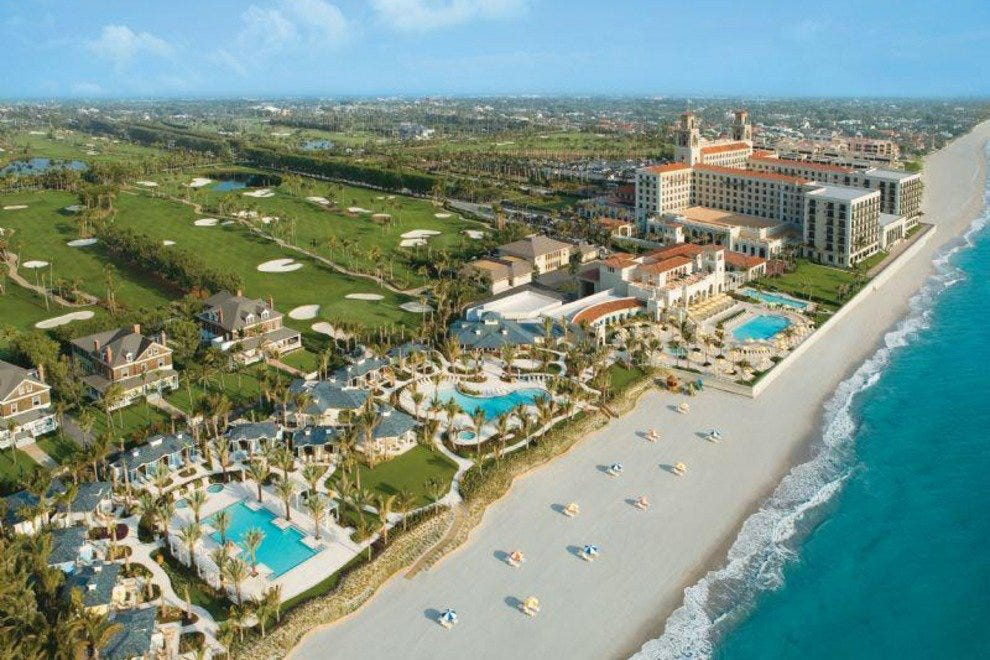
\includegraphics[width=160mm]{../data.png}
\caption{The original image \label{overflow}}
\end{figure}
After we convert and recolor it
\begin{figure}[H]
\centering
\includegraphics[width=160mm]{../ans2.png}
\caption{The recolored image \label{overflow}}
\end{figure}
We see that we can make out what it has done, but the quality of the image is no where near as good as it was. 

\subsubsection{How could you measure the quality of the final result}
The way I measure the quality of the final result is through a specific loss function. 
\begin{center}
L = $\frac{\sqrt{\sum_{i = 0}^{width} \sum_{j=0}^{height}(y[i][j] - x[i][j])^2}}{i*j}$
\end{center}
Basically we find the deviation from the actual RGB value and get the root mean square value. The loss of this was 0.115. This value would make more sense when I describe the improved agent. 

I thought that the result was satisfying both visually and mathematically. 

\subsubsection{Bonus}
To find the most effective k I used the tried and trusted "Elbow Method."The Elbow Method can be described as the follows: Calculate the Within-Cluster-Sum of Squared Errors (WSS) for different values of k, and choose the k for which WSS becomes first starts to diminish. In the plot of WSS-versus-k, this is visible as an elbow.\\
Here is my plot for WSS (loss) versus k
\begin{figure}[H]
\centering
\includegraphics[width=160mm]{../effectiveKValue.png}
\caption{WSS v K\label{overflow}}
\end{figure}
We see that coincidentally the elbow k value is 5
\pagebreak
\subsection{The Improved Agent}
Here I try to build an improved agent. I try to approach this as a soft classification problem. I love probability and I thought it would be useful to try and use it here. First I will show the final results and then answer the questions.\\

This the original image. The same one as used for the basic agent. Following it is the recolorized image I get after running the improved agent.

\begin{figure}[H]
\centering
\includegraphics[width=160mm]{../ans9.png}
\caption{The recolored image \label{overflow}}
\end{figure}

\subsubsection{A specification of your solution, including describing your input space, output space, model space, error or
loss function, and learning algorithm. For instance, do you want to attempt this as a classification
problem (as in the basic agent) or a regression problem, or some kind of soft classification?}
The input space is the whole gray scale image and the colorized left side of the image. The output space is the colorized right side of the image. The model space is the left rgb values. The loss function is the same as K clustering where we try to find centers that are most suitable to the data. \\
So the way I calculate the probability is I calculate the distance to the center of each  cluster. Then the probability is assigned in this way
\begin{center}
$P[C[i]] = 1/dist(C[i], color)$ then normalized
\end{center}
I then use these probabilities to pick which cluster I should use to color the image in. I choose the two highest probability colors and then do a weighted coin flip to find out the color I should choose. By doing this I try to eliminate the fact that two very similar colors can be switched when we go from grayscale to color. This results in a picture that is visually not that appealing but the numerical score is higher in terms of my loss function.\\
This effectively balances out the loss to be more or less the same. For eg if the color is too similar then instead of an all or nothing approach that can severely increase loss, we normalize by using probabilities.
\subsubsection{How did you choose the parameters (structure, weights, any decisions that needed to be made) for your model?}
The decision that I made was the select only the first most similar 3x3 gray patch and then use the representative color in the colored training image to find the probabilities. I also made the arbitrary decision of selecting the top two probabilities. 

\subsubsection{Any pre-processing of the input data or output data that you used.}
As far as preprocessing is concerned, I only calculated the average of the 3x3 gray scale on the testGrayScale matrix. By doing this I could effectively find out the most representative gray color in the training data. 

\subsubsection{How did you handle training your model? How did you avoid overfitting?}
I trained it on my own computer. It is a relatively light weight model. I use kd trees to find the most similar 3x3 gray scale matrices and that helped a lot. In terms of overfitting this model would crash and burn when used on another image, but works pretty well on the same image. It also depends a lot on the colors that are already present in the image. Very similar and monotonous images are likely to give bad results. 

\subsubsection{An evaluation of the quality of your model compared to the basic agent. How can you quantify and qualify the
differences between their performance? How can you make sure that the comparison is ‘fair’?}

So I use the same quality function as I did on the basic agent. The score I got is 0.09. This is lower than the first one even though it visually looks worse. This comparison is fair because they are both the same image that were trained on two different models, with equal data available. 

\subsubsection{How might you improve your model with sufficient time, energy, and resources?}
I would try to train the model on more images and use more grayscale pixels to make a predictions or classify. It would also be interesting to see how the model would do if any of the arbitrary parameters would change like number of points selected, k value, and how I assign probabilities. 
\pagebreak
\section{Using Tensorflow and keras}

I first tried to do this using regression but the results were absolutely terrible. Here is the colored image. 

\begin{figure}[H]
\centering
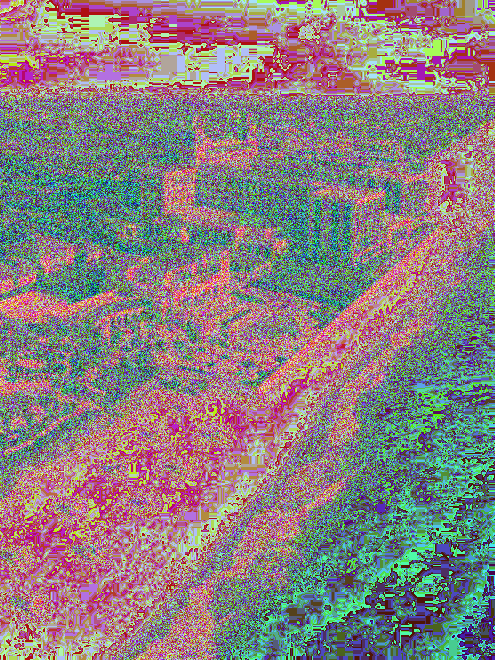
\includegraphics[width=70mm]{../pls.png}
\caption{The grayscale image \label{overflow}}
\end{figure}
I figured out that using linear regression was not the way. Though you can figure out what the image is, but the colors are all over the place. The loss score is also very big 0.23. So I decided to research on the internet and piece together a solution. 
\\

In this section I use TensorFlow and Keras to use auto-encoders and decoders to try and colorize an image. 

\subsection{What is an auto-encoder}
Autoencoder is an unsupervised artificial neural network that learns how to efficiently compress and encode data then learns how to reconstruct the data back from the reduced encoded representation to a representation that is as close to the original input as possible. - https://towardsdatascience.com/auto-encoder-what-is-it-and-what-is-it-used-for-part-1-3e5c6f017726 \\

Here I try to "trick" the autoencoder by putting a black and white picture as the input and same color picture as output and tell the algorithm that they are the same image. It then automatically changes it's biases and weights through training steps to be able to classify and assign images color.

\subsection{Dataset}
The dataset I used was the stanford dog data set. It contains images of various dogs. 150 images per dog. I only trained on 1 dog but to get good results one could train on a lot more breeds of dogs. Here is the link of the dataset - http://vision.stanford.edu/aditya86/ImageNetDogs/
\subsection{Results}
Since I did not have the computing power I could not train the model for too long. 5 epochs was all my computer could handle and hence the results are not too good. Here is an example. 

\begin{figure}[H]
\centering
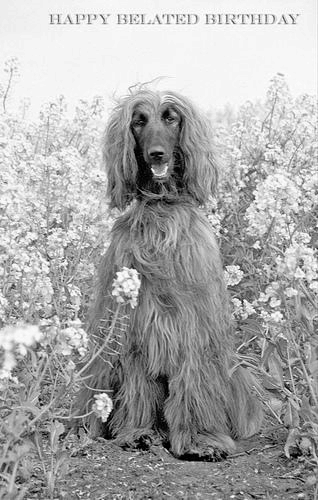
\includegraphics[width=70mm]{../please.png}
\caption{The grayscale image \label{overflow}}
\end{figure}

\begin{figure}[H]
\centering
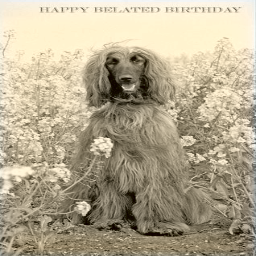
\includegraphics[width=70mm]{../result.png}
\caption{The recolored image \label{overflow}}
\end{figure}

\subsection{RGB - LAB}
Through my research I saw that converting to LAB was way more effective in terms of training this model. This reduced the number of features and also made for an efficient way to convert images to gray scale for training. 

\subsection{Activation Function}
For the activation function I used relu and for the last one I use tanh. Relu goes from 0 to 1 and was effective for gray scale images but since AB values can be negative I used tanh for the last layer that goes from -1 to 1

\subsection{Improvements}
More training data will definitely help with better image colors. 

\subsection{Citations}
I had tremendous help from the following resources \\

\begin{itemize}
\item https://towardsdatascience.com/auto-encoder-what-is-it-and-what-is-it-used-for-part-1-3e5c6f017726
\item https://towardsdatascience.com/image-colorization-using-convolutional-autoencoders-fdabc1cb1dbe
\item https://www.youtube.com/watch?v=EujccFRio7o
\end{itemize}

\end{document}